\documentclass{article}

\usepackage[preprint]{neurips_2024}

\usepackage[utf8]{inputenc}
\usepackage[T1]{fontenc}
\usepackage{hyperref}
\usepackage{url}
\usepackage{booktabs}
\usepackage{array}
\usepackage{tabularx}
\usepackage{graphicx}
\usepackage{amsfonts}
\usepackage{nicefrac}
\usepackage{microtype}
\usepackage{xcolor}

\graphicspath{{figures/}}


\title{CNNs vs.\ Vision Transformers: Pretraining and Data Augmentation for Multi-Label Image Classification}


\author{%
  DS6050 Group 8 \\
  University of Virginia \\
  Brady Genz, Chloe Merriweather, Alyssa Samuel, Sam Park \\
}


\begin{document}

\maketitle

\begin{abstract}
We compare convolutional neural networks (CNNs) and vision transformers (ViTs) on multi-label image classification, focusing on how pretraining and data augmentation shape their performance and data efficiency. Using the PASCAL VOC 2012 benchmark, we evaluate two CNNs (ResNet-50, ConvNeXt-T) and two transformer-based models (ViT-B/16, DeiT-S) across both training-from-scratch and ImageNet-pretrained conditions, varying the training data fraction from 5\% to 100\%. We find that ImageNet pretraining substantially improves performance for all four architectures and reverses which model performs best, with the CNN family leading from scratch and the transformer family leading after pretraining. ConvNeXt-T, despite being a CNN, depends more heavily on pretraining than ResNet, suggesting its transformer-era design choices mostly pay off when pretraining is part of the recipe. Data augmentation, by contrast, has only a small effect on pretrained fine-tuning at this scale, and our findings on this multi-label dataset closely follow the broader CNN-vs-transformer literature even though that literature is mostly based on single-label work. Code is available at \url{https://github.com/sanghoonio/image-cnn-transformers}.
\end{abstract}


\section{Introduction}

Deep learning has significantly advanced image classification, with convolutional neural networks (CNNs) and Vision Transformers (ViTs) emerging as the dominant architectural paradigms. CNNs, such as ResNet, incorporate strong inductive biases like locality and translation equivariance, allowing them to learn effectively even with limited training data. In contrast, Vision Transformer models rely on self-attention mechanisms to capture global relationships across image patches, often achieving superior performance when trained on large-scale datasets. However, this advantage typically depends on extensive pretraining and large amounts of labeled data, raising important questions about their effectiveness in data-constrained environments.

While prior work has extensively compared CNNs and transformers on single-label benchmarks such as ImageNet, multi-label classification introduces additional complexity, as models must capture both local features and contextual relationships across multiple classes simultaneously. Despite its practical importance, the behavior of CNNs and ViTs under multi-label settings, particularly with varying levels of data availability and augmentation, remains less explored. To address this gap, we evaluate these architectures on the multi-label PASCAL VOC benchmark, focusing on how pretraining and data augmentation influence performance and data efficiency across different training regimes.


\section{Methodology}

\subsection{Dataset}

We use PASCAL VOC 2012 (5,717 train / 5,823 val images, 20 classes, avg.\ 1.46 labels/image). To study data scaling, we construct training subsets at 5\%, 10\%, 20\%, 50\%, and 100\% of training data using iterative stratification (\texttt{scikit-multilearn} \texttt{IterativeStratification}) to preserve multi-label class distributions. Each configuration is run with 3 random seeds; results report mean~$\pm$~std mAP.

\subsection{Model Architectures}

We evaluate two architectures per family. For CNNs: \textbf{ResNet-50} (classical residual CNN with $3 \times 3$ kernels and built-in locality and translation equivariance) and \textbf{ConvNeXt-T} (modernized CNN with $7 \times 7$ depthwise convolutions, GELU activations, and transformer-era training recipes). For transformers: \textbf{ViT-B/16} ($16 \times 16$ patch tokens processed by 12 attention blocks, no spatial inductive bias) and \textbf{DeiT-S} (smaller ViT trained with CNN-teacher distillation, injecting implicit spatial priors). All models replace their original classification head with a 20-logit linear layer for multi-label prediction.

\begin{table}[h]
\centering
\caption{Evaluated architectures.}
\smallskip
\begin{tabular}{llll}
\toprule
\textbf{Architecture} & \textbf{Family} & \textbf{Params} & \textbf{Key Feature} \\
\midrule
ResNet-50   & CNN         & $\sim$25M & Residual blocks, $3 \times 3$ conv, locality bias \\
ConvNeXt-T  & Modern CNN  & $\sim$29M & $7 \times 7$ depthwise conv, GELU, LayerNorm \\
ViT-B/16    & Transformer & $\sim$86M & $16 \times 16$ patches, 12 attention blocks \\
DeiT-S      & Transformer & $\sim$22M & CNN-distilled, data-efficient transformer \\
\bottomrule
\end{tabular}
\label{tab:architectures}
\end{table}

\subsection{Pretraining Conditions}

\textbf{Pretrained:} ResNet-50 and ConvNeXt-T use ImageNet-1K weights (\texttt{torchvision}). ViT-B/16 uses the \texttt{augreg\_in21k} checkpoint (ImageNet-21K, \texttt{timm}). DeiT-S uses its standard ImageNet-1K distillation checkpoint. Note that ViT-B/16's pretrained checkpoint was trained on roughly 10$\times$ more images than the CNN baselines, which may independently contribute to its pretrained performance. \textbf{From scratch:} All models are also trained from random initialization on VOC only, isolating architectural data efficiency from transfer learning.

\subsection{Training}

\textbf{Loss:} \texttt{BCEWithLogitsLoss} (sigmoid + binary cross-entropy per class). \textbf{Optimizer:} AdamW (weight decay 1e-2) with differential learning rates for pretrained models (CNN backbone 1e-4 / head 1e-3; ViT backbone 1e-5 / head 1e-3) and uniform rates for scratch (CNN 1e-2, ViT 1e-3). \textbf{Schedule:} Cosine annealing over the training horizon, with a 5-epoch linear warmup for from-scratch transformers. \textbf{Early stopping:} patience $=$ 5 epochs on validation mAP. All inputs are $224 \times 224$ with ImageNet normalization.

\subsection{Data Augmentation}

We test three policies on the two best pretrained models at 100\% data to assess whether augmentation benefits transformers more than CNNs:
\begin{enumerate}
    \item \textbf{None} --- resize and normalize only;
    \item \textbf{Standard} --- \texttt{RandomResizedCrop}, \texttt{HorizontalFlip}, \texttt{ColorJitter} (brightness/contrast/saturation $=$ 0.4, hue $=$ 0.1);
    \item \textbf{Strong} --- standard plus \texttt{RandAugment} (2 ops, magnitude 9)~\citep{cubuk2019randaugment}.
\end{enumerate}
Test-time transform is always \texttt{Resize(256)} $+$ \texttt{CenterCrop(224)} $+$ normalize.

\subsection{Evaluation}

The primary metric is mAP: the unweighted mean of per-class Average Precision across all 20 VOC classes, computed via \texttt{sklearn}'s \texttt{average\_precision\_score} on sigmoid-transformed logits. We additionally report per-class AP across all 20 classes. Computational efficiency (parameter count and training time) is reported for all four architectures.

\subsection{Experimental Design}

Core scaling experiment: 4 architectures $\times$ 2 pretraining conditions $\times$ 5 data fractions $\times$ 3 seeds $=$ 120 runs. Augmentation ablation: 2 models $\times$ 2 additional policies (none, strong) $\times$ 1 fraction $\times$ 3 seeds $=$ 12 additional runs (the standard policy reuses the core-sweep runs at 100\% data). All experiments were run on the UVA Rivanna HPC cluster, with one NVIDIA GPU allocated per job.

\begin{table}[h]
\centering
\caption{Experimental design summary.}
\smallskip
\begin{tabular}{llr}
\toprule
\textbf{Experiment} & \textbf{Conditions} & \textbf{Runs} \\
\midrule
Core scaling        & 4 arch $\times$ 2 pretraining $\times$ 5 fractions $\times$ 3 seeds & 120 \\
Augmentation ablation & 2 models $\times$ 2 add'l policies $\times$ 1 fraction $\times$ 3 seeds & 12  \\
Per-class AP analysis & 20 classes $\times$ 4 arch $\times$ 2 pretraining                          & --- \\
Efficiency comparison & Param count and training time, all 4 models                                  & --- \\
\bottomrule
\end{tabular}
\label{tab:experiments}
\end{table}


\section{Results}

The ConvNeXt-T, DeiT-S, ResNet-50, ViT-B/16 image classification models evaluated 11,000 PASCAL VOC images across 20 objects under different training conditions. The model that performed the best was determined by comparing the mAP (mean Average Precision) metric among the models and objects. The results show a very consistent ranking across model families with ViT-B/16 and ConvNeXt-T as the top performers followed by DeiT-S and lastly and ResNet-50. The results determined that the best-performing model type of ViT-B/16 achieved the best mAP overall 0.927 as referenced in Figure 1, and leads in the low-data regime (0.81 at 5 percent data). This model showed the highest accuracy and strongest consistency in comparison to the other models with an average of 0.744 mAP. ConvNeXt-T had a good pretrained performance, but the scratch runs brought down the overall average to 0.566. Similarly, DeiT-S model’s results showed a strong pretrained performance, but weaker results for the scratch runs with an average of 0.553 mAP. Lastly, the model that performed the worse was the ResNet-50, which had the lowest average of 0.487 mAP among the models.

The pre-trained data outperformed the data from scratch. Models trained from scratch ranged from approximately 0.10–0.29 mAP with full data, while pretrained models start at ~0.76 mAP. For the highest performing model of ViT-B/16, the average pretrained mAP showed a result of 0.895 while the average scratch mAP was 0.165. The improved performance range gained from pre-training was significant across all models, with the ConvNeXt-T model showing the most improvement of + 0.757. All earliest best epochs during the run came from the scratch models, but the pretrained models peaked much later as more epochs ran. The ConvNeXt-T model from scratch showed the strongest results in the first few epochs.

The percentage or fraction of data impacted each of the model’s performance among the runs. At 5 percent data, the average mAP was 0.44 across the models, which represented the widest gap between runs. Pretrained models were around 0.76–0.81, while scratch models performed at 0.08–0.12. 10 percent of data showed an average mAP of .48, while 20 percent data showed an average of .50 mAP and 100 percent data produced an average of .66. The accuracy improved with the runs with 100 percent data for the models. However, 20 percent of the data was the most efficient as pretrained models were already in the 0.82–0.89 range producing a solid performance with a fifth of the dataset.

The results from the experiment showed varying performances across the object classes. The object classes that performed the best were aeroplane, cat, train, sheep, horse, dog, bird, cow with an AP > 0.98. These all share a common trait of having a strong, consistent silhouette with little visual ambiguity within the images. Based on the data, the aeroplane had the highest average AP at 0.9954 across the best-performing runs (pretrained ViT-B/16, 100 percent data).The middle range group had an AP 0.88–0.96, which included the person, bus, motorbike, boat, bicycle, tv monitor, and car. The bottom range of objects with an AP < 0.84 was the chair, sofa, dining table, bottle, and potted plant. All models struggled with identifying smaller or more complex objects.

\begin{figure}[h]
    \centering
    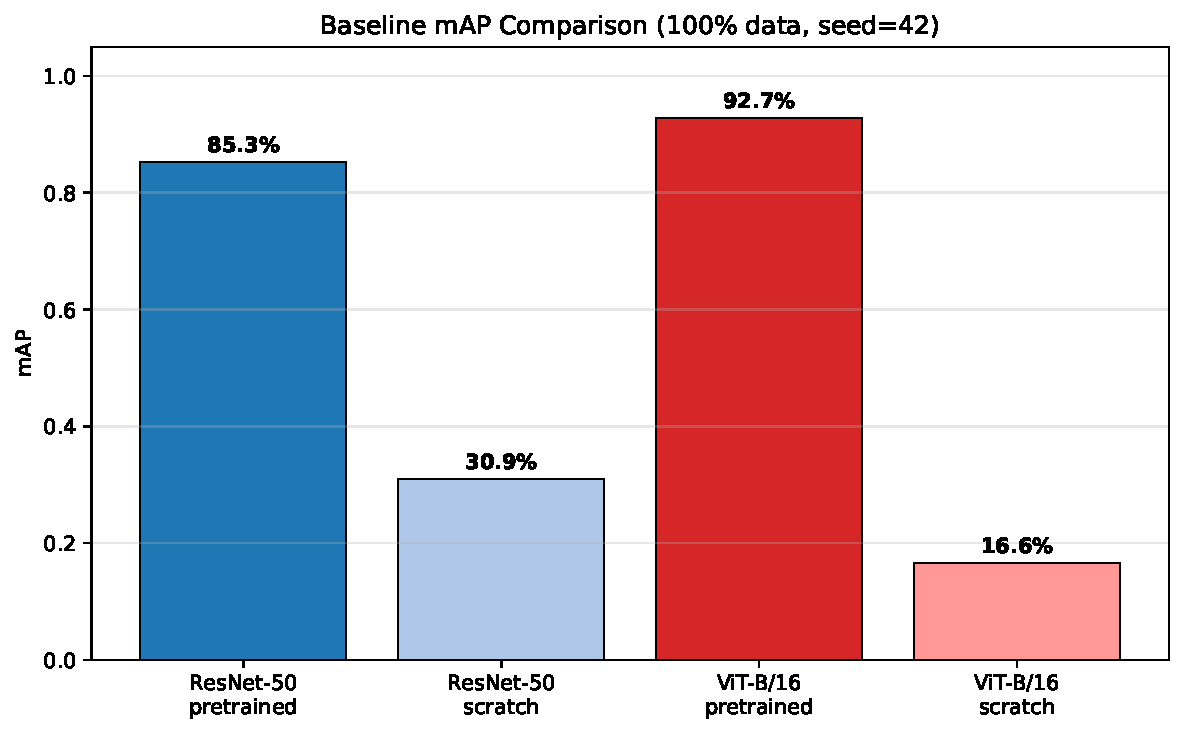
\includegraphics[width=0.85\textwidth]{mAP_comparison}
    \caption{mAP by architecture and pretraining condition (100\% data, mean $\pm$ std over 3 seeds). Pretrained bars use solid colors; from-scratch bars are lighter.}
    \label{fig:map_comparison}
\end{figure}


\begin{figure}[h]
    \centering
    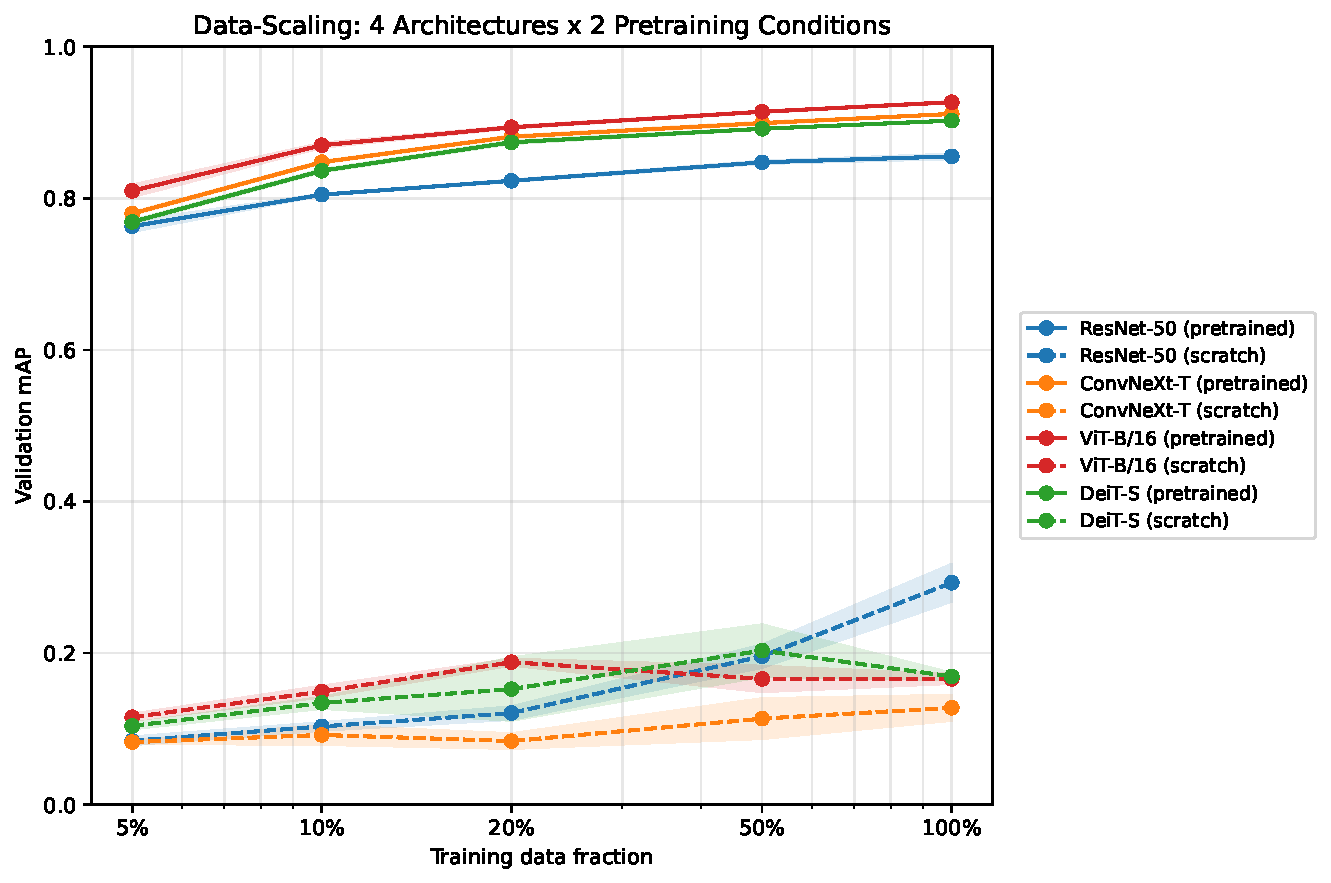
\includegraphics[width=0.85\textwidth]{data_scaling}
    \caption{Validation mAP versus training data fraction across the four architectures and two pretraining conditions.}
    \label{fig:data_scaling}
\end{figure}

\begin{figure}[h]
    \centering
    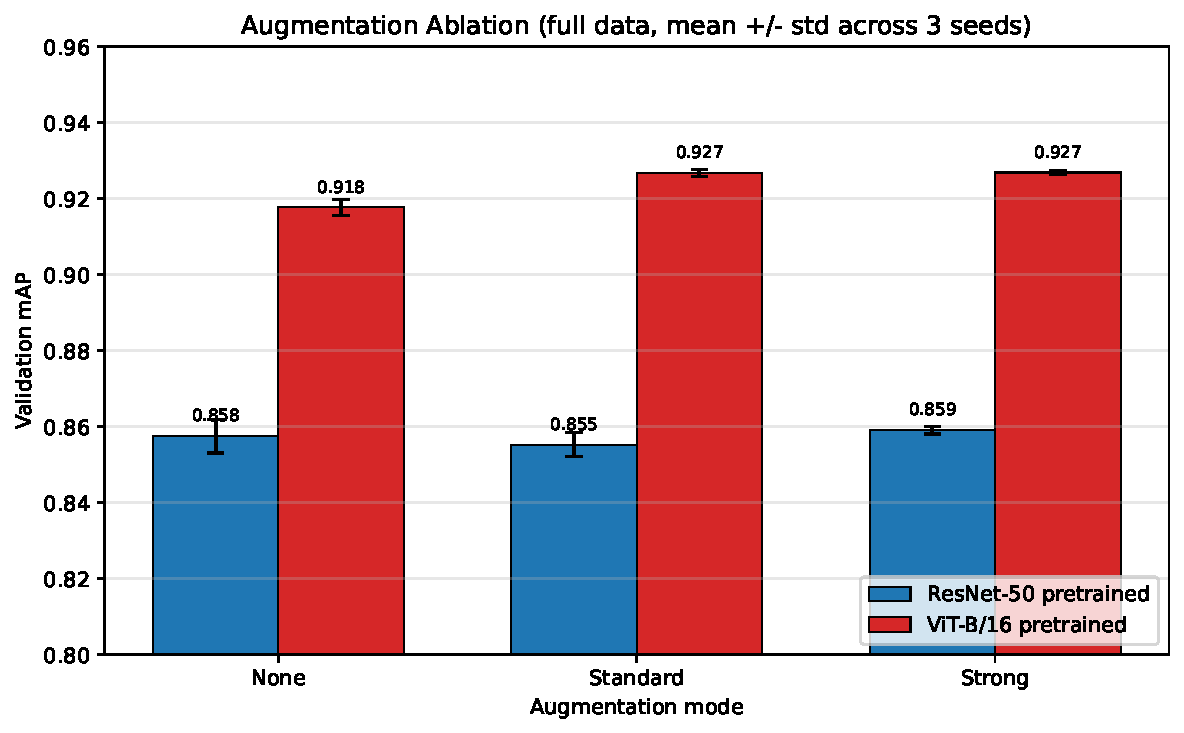
\includegraphics[width=0.7\textwidth]{augmentation_ablation}
    \caption{Augmentation ablation on pretrained ResNet-50 and ViT-B/16 at full data (3 seeds).}
    \label{fig:augmentation_ablation}
\end{figure}

\begin{figure}[h]
    \centering
    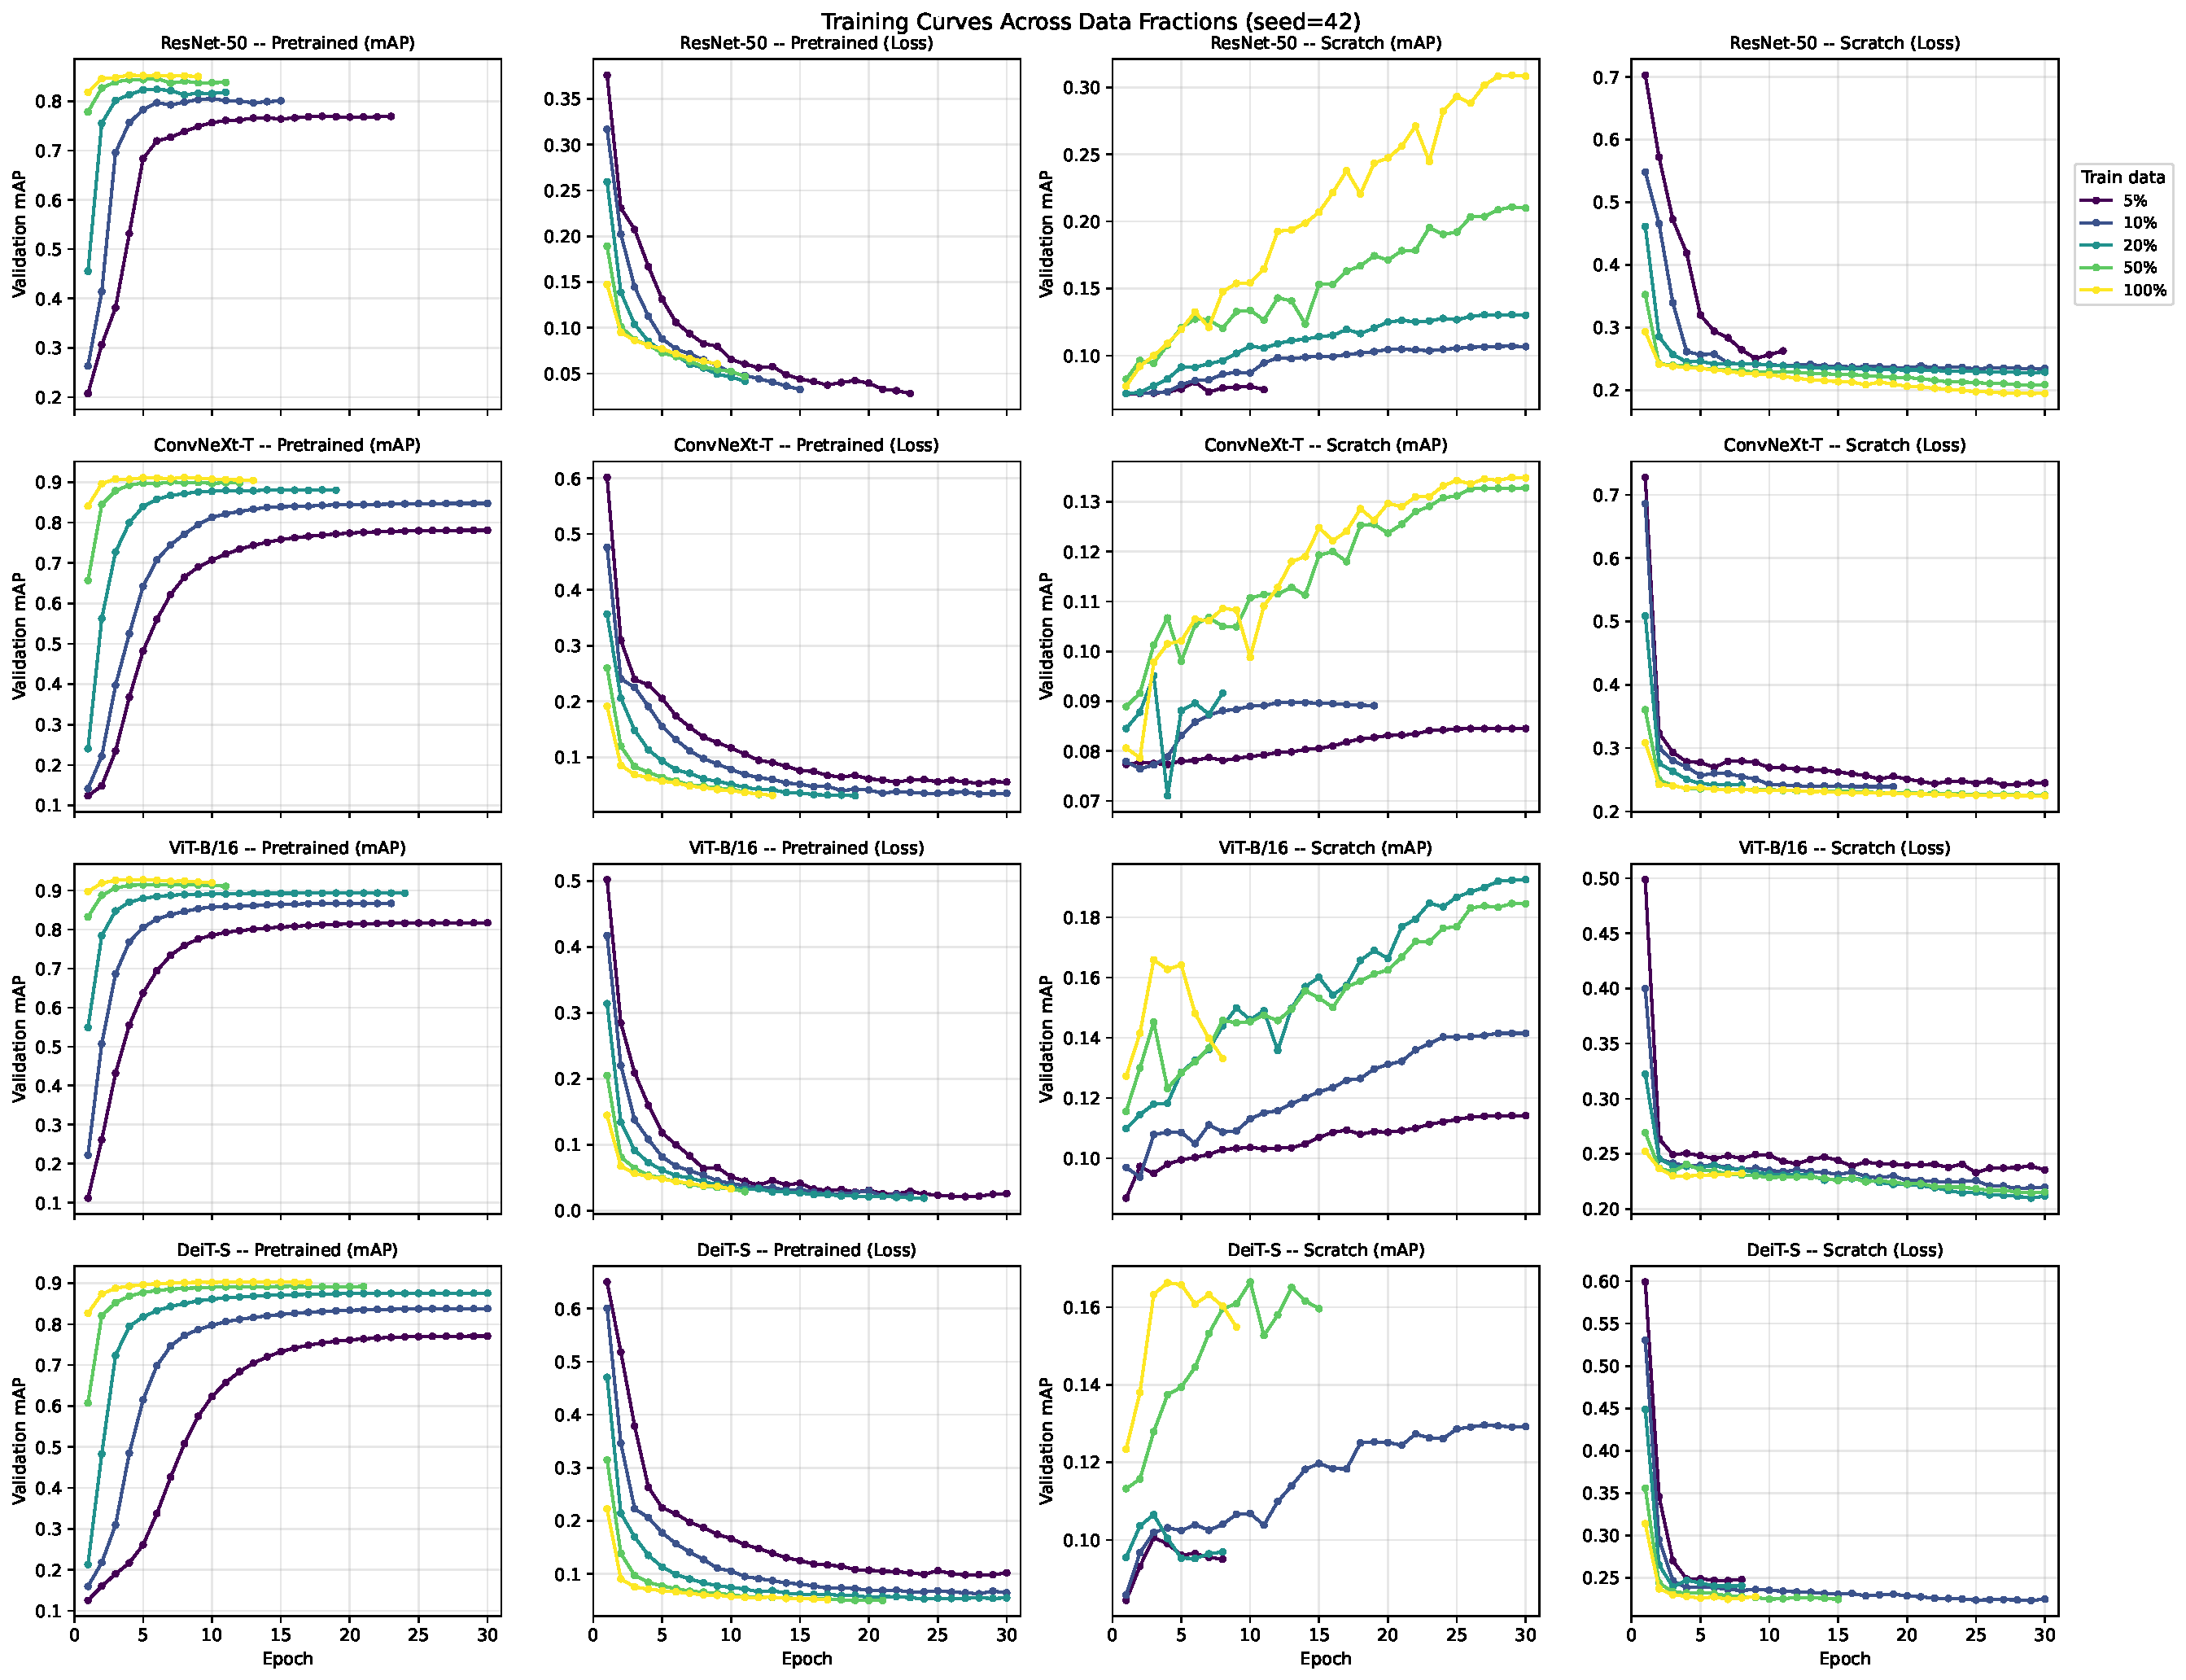
\includegraphics[width=\textwidth]{training_curves_fractions}
    \caption{Validation mAP and training loss versus epoch across the five data fractions, broken out by architecture and pretraining condition (seed=42). Lines that end before epoch 30 indicate early stopping fired. From-scratch ViT-B/16 and DeiT-S complete the full schedule at small and moderate data fractions but trigger early stopping at the largest fraction; the from-scratch CNNs run the full schedule at every fraction.}
    \label{fig:training_curves_fractions}
\end{figure}


\section{Analysis}

Our results provide four findings that help answer our primary research
question. First, pretraining substantially improves model performance
for all four architectures, but reverses which model type performs best
at higher training data fractions. Second, ConvNeXt-T, despite being a
CNN, substantially underperforms ResNet and even transformers when
training from scratch, suggesting it is not simply an improved CNN.
Third, data augmentation has minimal effects on performance for models
trained from scratch at these levels of training data, and a small
effect independent of augmentation strength for pretrained models.
Lastly, our findings on this multi-label dataset closely follow the
broader CNN-vs-transformer literature, which is mostly based on
single-label work, suggesting that the architectural conclusions from
single-label settings extend to multi-label classification at this
scale.

The first of our findings is largely as expected per the literature:
transformers perform poorly compared to CNNs when trained on smaller
datasets, but can outperform them with enough pretraining. For models
trained from scratch, our results show ResNet outperforming DeiT-S and
ViT by almost a factor of two, while with ImageNet pretraining, ViT
leads, followed by ConvNeXt-T, DeiT-S, and then ResNet notably last.
These findings closely follow results from \citet{dosovitskiy2021}, who
originally identified that without sufficient pretraining data, ViTs
suffer from the absence of translation equivariance and locality. On
the other hand, with sufficient examples, attention mechanisms can
generalize and approximate the innate features of CNNs to the point of
outperforming them where the features being hard coded may reduce the
capacity to learn edge cases. Our results here validate these earlier
findings with a dataset roughly two orders of magnitude smaller than
ImageNet-1K as floor-level evidence of the weaknesses of transformer
models with smaller training sets. It is also worth noting that ViT-B/16's
pretrained checkpoint comes from ImageNet-21K rather than ImageNet-1K,
which is roughly an order of magnitude more pretraining images than the
CNN baselines. This may contribute to its pretrained lead beyond
architecture alone.

Breaking down the from-scratch training performance across data
fractions in a bit more detail, we see that ResNet improves
monotonically across all five fractions, with the largest gains at the
higher fractions, suggesting it is still on its scaling curve and would
benefit from additional training data if resources allow. It, alongside
ConvNeXt, completes its full 30-epoch training schedule at higher data
fractions. On the transformer side, the learning trajectories are
rather underwhelming. At the highest data fractions, neither
transformer is able to reach even 10 epochs due to early stopping
(Figure~\ref{fig:training_curves_fractions}).
Previous literature by \citet{touvron2021} advises using warmup epochs
for transformers, which we attempted to implement with a five-epoch
linear warmup prior to cosine annealing. This appears to work at lower
data fractions where mAP rises through warmup and the entire 30-epoch
schedule. Though the performance at these fractions straggles behind
that of ResNet, they do indicate learning. At the highest data
fractions, mAP peaks in the warmup phases and decays shortly
afterwards, leading to early stopping only at around epochs 8 and 9.
The full method by \citet{touvron2021} included more controls such as
distillation, strong augmentation, and a much longer epoch schedule to
support training on ImageNet-1K, a much larger dataset. As such, our
results for transformers reflect also the difficulty of properly tuning
the training regimen compared to CNNs.

ConvNeXt showed a very peculiar result when comparing the pretrained to
the from-scratch results. Though it is a CNN like ResNet, with
pretraining it outperformed DeiT and was very close to ViT. Trained
from scratch, it performed worse than all other models at the highest
data fraction. This suggests that the design elements specific to
ConvNeXt inspired by transformers may not always be helpful. Some of
these elements include $7 \times 7$ depthwise kernels compared to
ResNet's $3 \times 3$, GELU instead of ReLU activations, LayerNorm in
place of BatchNorm, fewer activation and normalization layers per
block, and inverted bottleneck designs. These changes give the model
more capacity, but they also weaken the locality and translation
equivariance that vanilla ResNet relies on. With
pretraining, that trade-off works in ConvNeXt's favor: the added
capacity gets filled with features learned during pretraining, and the
model performs well. Without pretraining, the trade-off goes the other
way. ConvNeXt has more parameters than ResNet but less of the inductive
bias that helps it learn from a small training set. This matches the
broader argument by \citet{liu2022} that CNNs can match transformers
given modern training recipes, though our scratch results add a
qualification: this seems to hold mostly when pretraining is part of
the recipe. Within the CNN family, ResNet and ConvNeXt are trained with
the same recipe, but the gap between pretrained and from-scratch
performance is more than twice as wide for ConvNeXt as for ResNet. The
design changes that help ConvNeXt approach transformer performance with
pretraining are the same ones that hurt it from scratch.

As for augmentation, though \citet{steiner2022} claim that augmentation
can substitute an order of magnitude of training data, we found that it
did not substantially improve training performance across any of the
models tested at any data fraction. For ResNet, the effect of moving
across the three augmentation tiers is within seed noise. For ViT,
there is a small gain of about one point from no augmentation to
standard, then a plateau at strong. On the other hand, going from
10\% to 100\% of the training set, which is an order of magnitude,
increases the mAP by about six points. At these scales, it is likely
that augmentation is not enough to substantially create enough
variation in the data for the models to be able to generalize from
them. Despite the magnitude difference, ViT benefiting slightly and
ResNet not at all is still consistent with the observation that ViTs
are more augmentation-sensitive than CNNs.

Lastly, one of our motivations for using this dataset was to consider
learning on multi-label co-occurrence frequencies, and whether this
would have any notable effect on findings. We treat the task as a
genuine multi-label problem using independent sigmoid outputs, binary
cross-entropy loss, iterative stratification of training subsets to
preserve co-occurrence rates across data fractions, and macro-averaged
per-class AP for evaluation. Despite this setup, our findings closely
follow the single-label literature: the pretraining flip, the ConvNeXt
paradox, and the augmentation results all match what would be expected
from single-label work. We did not pursue multi-label-specific analyses
such as class groupings (e.g., texture- versus context-dependent
classes) or co-occurrence pattern attribution, which remain open for
follow-up.


\section{Future Work}

While this study provides a comparative evaluation of CNNs and Vision Transformers on multi-label image classification using PASCAL VOC, several opportunities remain for extending the analysis and improving the experimental framework. One important direction is scaling the experiments to larger and more diverse datasets such as MS COCO or medical imaging benchmarks. PASCAL VOC is valuable for studying low-resource and multi-label behavior, but its relatively small size and limited number of classes may constrain the generalization of conclusions regarding transformer scalability and representation learning. Evaluating the same architectures on larger datasets would allow investigation of whether the observed trends in pretraining and data efficiency persist under more realistic large-scale conditions.

Another promising extension is the exploration of hybrid CNN-transformer architectures. Recent work suggests that combining convolutional inductive biases with transformer self-attention can improve both efficiency and robustness, particularly in resource-constrained settings. Architectures such as ConvNeXt already demonstrate that many transformer-era training techniques can significantly improve convolutional models, narrowing the historical gap between CNNs and ViTs. Future experiments could therefore include hybrid or hierarchical architectures such as Swin Transformer, CMT, or iFormer to better understand how local and global feature representations interact in multi-label classification tasks.

Future work could also investigate more advanced training paradigms beyond supervised ImageNet pretraining. In recent years, self-supervised and multimodal approaches such as CLIP have demonstrated strong transferability and robustness across downstream computer vision tasks. Evaluating whether these pretraining strategies improve low-data performance on PASCAL VOC would provide additional insight into how representation learning influences transformer and CNN behavior under limited supervision. Similarly, longer training schedules, larger augmentation policies, label smoothing, Mixup, CutMix, and stochastic depth could be systematically evaluated to determine whether differences between CNNs and ViTs are architectural or primarily driven by optimization strategy.

Another important area for future investigation is robustness and generalization under distribution shifts. Prior studies have shown that CNNs and ViTs differ substantially in calibration, transferability, texture bias, and robustness to corrupted or adversarial inputs. Extending this project to include corrupted-image benchmarks, synthetic perturbations, occlusions, or adversarial attacks would provide a more complete characterization of model behavior beyond mean Average Precision alone. Since many real-world applications involve noisy and imperfect visual environments, robustness evaluation would strengthen the practical relevance of the findings.

Finally, future work should expand the interpretability and efficiency analysis of these architectures. While this project compares training time and parameter counts, further work could incorporate attention visualization, Grad-CAM analysis, feature similarity comparisons, and representation probing to better understand how CNNs and transformers learn contextual information differently. Recent hybrid mobile transformer models suggest that balancing local convolutional operations with efficient global attention may provide an effective tradeoff between accuracy and computational cost. Together, these directions would broaden the scope of the project and provide a more comprehensive understanding of how modern vision architectures behave across diverse data, training, and deployment conditions.


{\small

\begin{thebibliography}{9}

\bibitem[Cubuk et al.(2020)]{cubuk2019randaugment}
Cubuk, E.~D., Zoph, B., Shlens, J., \& Le, Q.~V. (2020).
\newblock RandAugment: Practical automated data augmentation with a reduced search space.
\newblock \textit{Advances in Neural Information Processing Systems 33 (NeurIPS 2020)}.

\bibitem[Dosovitskiy et al.(2021)]{dosovitskiy2021}
Dosovitskiy, A., Beyer, L., Kolesnikov, A., Weissenborn, D., Zhai, X., Unterthiner, T., \ldots\ \& Houlsby, N. (2021).
\newblock An image is worth 16x16 words: Transformers for image recognition at scale.
\newblock \textit{ICLR 2021}.

\bibitem[Liu et al.(2022)]{liu2022}
Liu, Z., Mao, H., Wu, C.~Y., Feichtenhofer, C., Darrell, T., \& Xie, S. (2022).
\newblock A ConvNet for the 2020s.
\newblock \textit{CVPR 2022}.

\bibitem[Steiner et al.(2022)]{steiner2022}
Steiner, A., Kolesnikov, A., Zhai, X., Wightman, R., Uszkoreit, J., \& Beyer, L. (2022).
\newblock How to train your ViT? Data, augmentation, and regularization in vision transformers.
\newblock \textit{Transactions on Machine Learning Research}.

\bibitem[Touvron et al.(2021)]{touvron2021}
Touvron, H., Cord, M., Douze, M., Massa, F., Sablayrolles, A., \& J\'egou, H. (2021).
\newblock Training data-efficient image transformers \& distillation through attention.
\newblock \textit{ICML 2021}.

\end{thebibliography}
}


\end{document}
